%! Author = Philipp Emmenegger
%! Date = 10/06/2021

\section{Declaring Types and Classes}
\subsection{Type Declarations}
\begin{itemize}
    \item New name for an existing type
    \item Can make other types easier to read
    \item Can have type parameters
    \item Can be nested
    \item Cannot be recursive
\end{itemize}
\begin{lstlisting}
type String = [Char]
-----------------------
type Pos = (Int, Int)
origin :: Pos
origin = (0, 0)

left :: Pos -> Pos
left (x,y) = (x-1, y)

-- Type parameter --
type Pair a = (a,a)
mult :: Pair Int -> Int
mult (m,n) ) m*n

-- Nested --
type Trans = Pos -> Pos
\end{lstlisting}

\subsection{Data Declarations}
\begin{itemize}
    \item Completely new type by specifying its values
    \item Values of new types can be used the same ways as built in types
    \item Constructors may also have parameters
    \item May also have type parameters
    \item Can be recursive
\end{itemize}
\begin{lstlisting}
data Bool = False | True
data Answer = Yes | No | Unknown

-- Parameter --
data Shape = Circle Float | Rect Float Float
square :: Float -> Shape
square n = Rect n n

-- Type parameters --
data Maybe a = Nothing | Just a

-- Recursive --
data Nat = Zero | Succ Nat
Succ (Succ (Succ Zero)) = 3
\end{lstlisting}

\subsection{Newtype Declarations}
If a new type has a \textbf{single constructor} with a \textbf{single element}, it can be declared using the \textit{newtype} mechanism.
For example, a type of natural numbers:
\begin{lstlisting}
newtype Nat = N Int
\end{lstlisting}

\subsection{Polymorphism}
\begin{enumerate}
    \item Ad-hoc Polymorphism: function with the same name denotes different implementations (function overloading / interfaces)
    \item Parametric Polymorphism: Code written to work with many possible types
    \item Subtype Polymorphism: one type can be substituted for another (subtype / supertype)
\end{enumerate}

\subsection{Type Classes}
\subsubsection{Class Declarations}
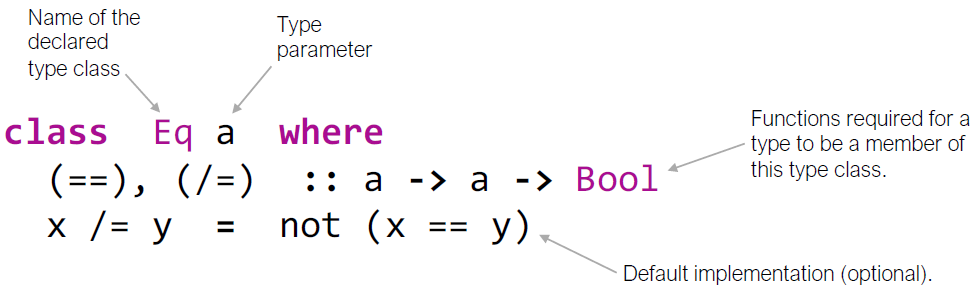
\includegraphics[width=0.8\linewidth]{img/class_declarations.png}\\
\subsubsection{Extending Classes}
 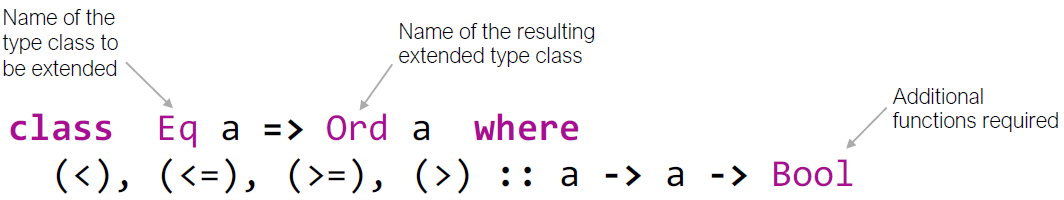
\includegraphics[width=0.9\linewidth]{img/type_classes_extend.png}
 \begin{itemize}
     \item All members of class \textit{Ord} are also members of type class \textit{Eq}
     \item Members of \textit{Ord} therefore also require \textit{(==)} to be defined
 \end{itemize}
 \subsubsection{Instance Declaration}
 A Type can be declared to be an instance of a type class using an instance declaration.\\
 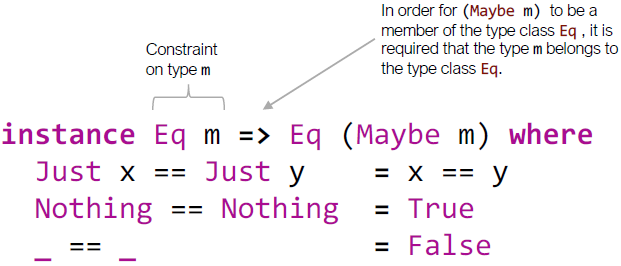
\includegraphics[width=0.8\linewidth]{img/instance_declaration.png}
 \subsubsection{Derived Instances}
 Default implementations for the built-in type classes \textit{Eq, Ord, Show, Read} can be generated automatically for \textbf{data} declarations using the \textbf{deriving keyword}:
 \begin{lstlisting}
data Bool = False | True
    deriving (Eq, Ord, Show, Read)
-- examples --
> False == False
True
> False < True
True
> show False
"False"
>read "False" :: Bool
False
\end{lstlisting}

\subsubsection{Type Constructors \& Kinds}
Type Constructors construct one type from another. This behaviour is expressed using kinds.
A kind is the type of a 'type'.\\
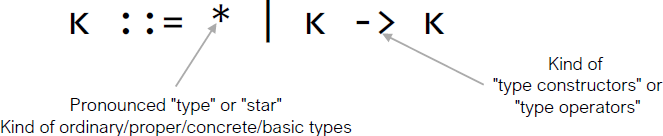
\includegraphics[width=0.7\linewidth]{img/type_constructors_kinds.png}\\
\textbf{Examples:}
\begin{lstlisting}
data Maybe a = Nothing | Just a
type Pair a = (a, a)
\end{lstlisting}

\subsubsection{Values, Types \& Kinds}
Only types of kind * can have a value.\\
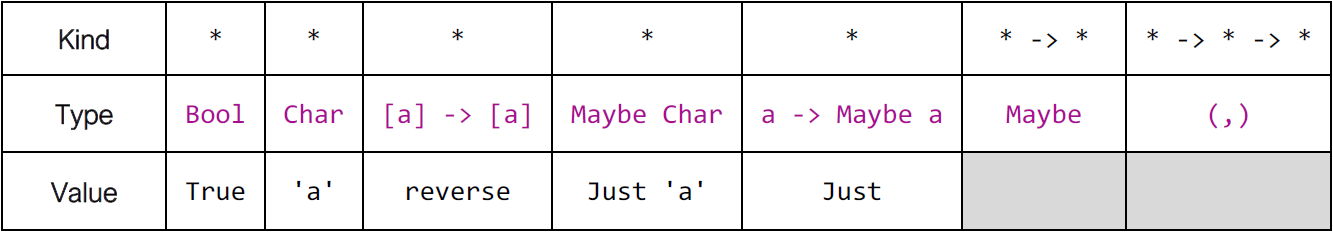
\includegraphics[width=\linewidth]{img/values_types_kinds.png}
\textbf{Why are Kinds useful?}\\
Just like how
\begin{itemize}
    \item Types are used to prevent the user from making errors at the value level
    \item Kinds are used to prevent the user from making errors at the type level
\end{itemize}

\subsection{Records}
Convenient syntax when data constructors have multiple parameters:\\
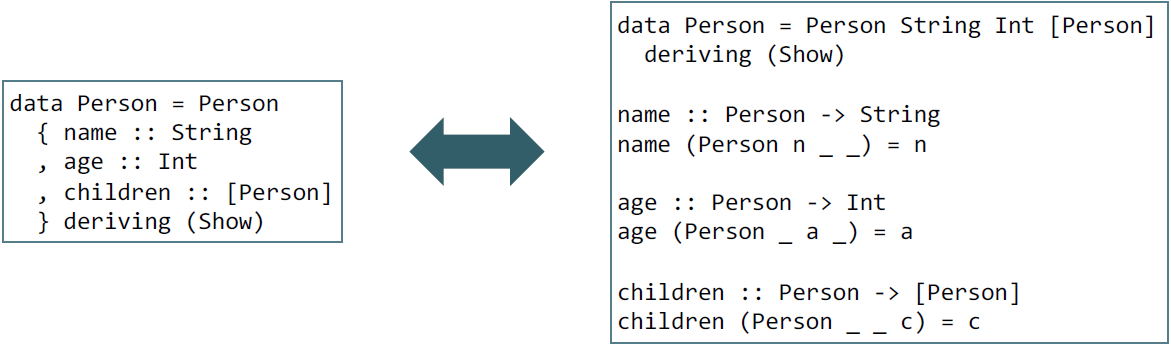
\includegraphics[width=\linewidth]{img/records.png}

\subsection{Modules}
\begin{itemize}
    \item Collection of related values, types, classes, etc.
    \item Name: Identifier that starts with a capital letter
    \item Naming convention for hierarchy: seperated using '.'
    \item Each module \textbf{Module.Name} must be contained in a file called \textbf{Module.Name.hs}
\end{itemize}
\textbf{Main Aims:}
\begin{itemize}
    \item Organising
    \item Defining visibility
\end{itemize}